\section{API}
\begin{frame}{API}
\begin{itemize}{}
\item \textbf{API} - \textit{Application Programming Interface}.
\item Es un conjunto de clases y m\'etodos que permiten comunicarse con otras otros programas, componentes o servicios.
\item La \textbf{API de Java} provee las funcionalidades necesarias para permitirnos utilizar sus caracter\'isticas o ventajas sobre los otros lenguajes.
\item Java cuenta con APIS para diversos objetivos, como por ejemplo, conectarse a un componente de Hardware, servicios en internet (sistemas de pago online), Comunicarse con tros lenguajes de programaci\'on, bases de datos, lenguajes de etiquetado (XML), etc.
\end{itemize}
\end{frame}

\begin{frame}{API}

\begin{block}{En general}
  Se conoce como API en java a un conjunto de librerias cuyos \textbf{imports} en nuestros programas nos ayudan a solucionar un problema de integraci\'on o comunicaci\'on espec\'ifico
\end{block}

\end{frame}


\begin{frame}{API - Ejemplo.}
  \begin{figure}
    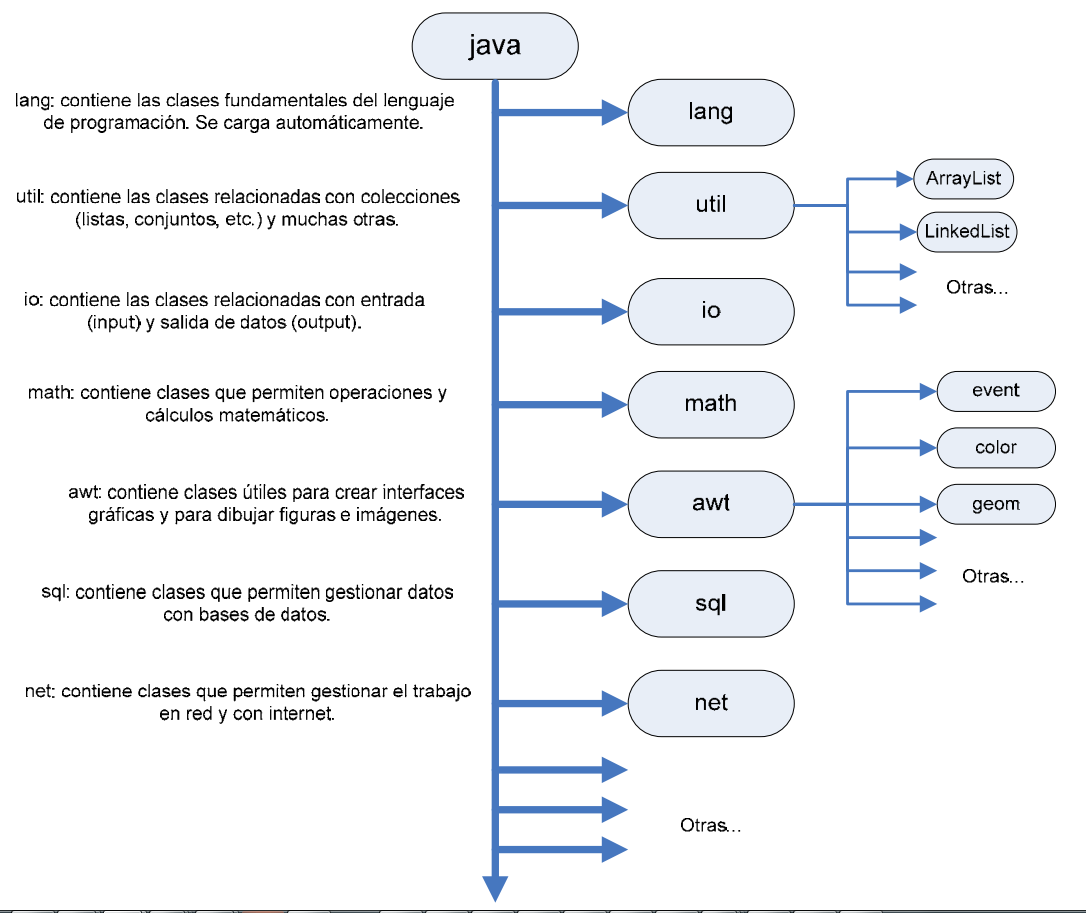
\includegraphics[scale=0.3]{figuras/API_Java.PNG}
  \end{figure}
\end{frame}

\begin{frame}{API - Ejemplo.}
  \begin{figure}
    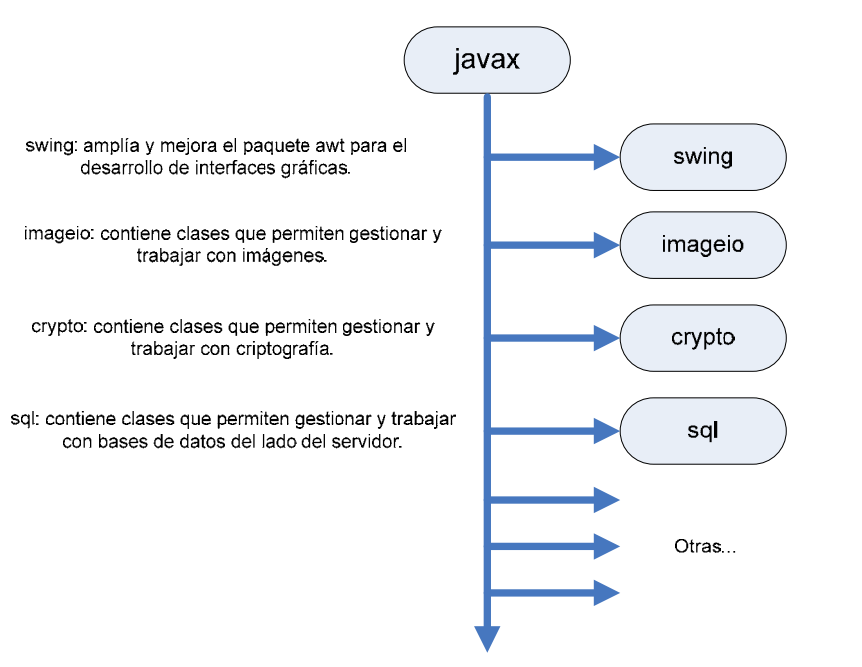
\includegraphics[scale=0.4]{figuras/API_Javax.PNG}
  \end{figure}
\end{frame}

\begin{frame}{Manejo de Excepciones - Declaraci\'on en m\'etodos}
	\begin{block}{Ejemplo.}
\lstinputlisting[language=Java,caption={},numbers=none]{resources/apis/Imports.java}
\end{block}
\end{frame}
